
\section{Tuning distance-dependency}

Stepping away, we 




Maybe simplicity of the model makes stuff wrong. Tune to Perin
distance profile.

Let 

In their study, \textcite{Perin2011} heavily rely on a
distance-dependent 


Here we introduce anisotropic networks tuned to reflect a given
distance-dependent connection profile. We face the following: Given
$C(x):[0,\sqrt{2}) \to [0,1]$, choose $w(x)$ such that the probability
to have a vertex is $C(x)$ $G_n,w$.

From ?? we have the relation ??. This however assumes . 

\[
C\left(\sqrt{x^2+w^2(x)}\right) = \frac{1}{\pi} \operatorname{arctan}
\frac{w(x)}{x}
\] 



Instead we propose the approximation $\sqrt{x^2 + w^2(x)} \approx  x$,
giving
\[
C(x) \approx \frac{1}{\pi} \operatorname{arctan} \label{eq:tanapprox}
\frac{w(x)}{x}.
\] 

This approximation holds well as long as $x \gg w(x)$.

  




\begin{figure}[htp]
  \centering
  \makebox{%
    \begin{overpic}[height=4.05cm]{%
        plots/6154302f.pdf}
      \put(85.5,57.5){\small\textbf{A}}
      %\put(12,5){\small\textbf{A}}
    \end{overpic}
    \hfill
    \begin{overpic}[height=4cm]{%
        plots/ef0e785d.pdf}
      \put(90.5,58.2){\small\textbf{B}}
    \end{overpic}
  }%
  \vspace{-0.15cm}
  \caption{ (\smtcite{6154302f}, \smtcite{ef0e785d})} %?? fix width issue!!
  \label{fig:determine_side_length}
\end{figure}

With side length 296:

% Mean:  0.115976056056
% Standard deviation:  0.00293436235458

from \smtcite{f11dca65}.


\begin{figure}[htp]
  \centering
  \makebox{%
    \begin{overpic}[width=0.5\textwidth]{%
        plots/875505b0_overall.pdf}
      \put(28,19){\small\textbf{A}}
    \end{overpic}
    \hfill
    \begin{overpic}[width=0.5\textwidth]{%
        plots/875505b0_single.pdf}
      \put(28,19){\small\textbf{B}}
    \end{overpic}
  }%
  \vspace{-0.6cm}
  \makebox{%
    \begin{overpic}[width=0.5\textwidth]{%
        plots/875505b0_recip.pdf}
       \put(28,19){\small\textbf{C}}
    \end{overpic}
    \vspace{-1cm}
    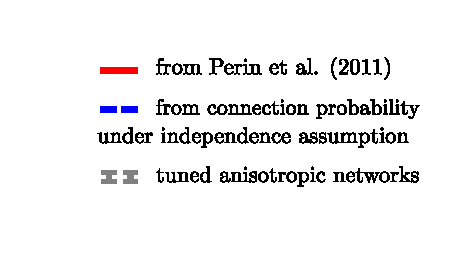
\includegraphics[width=0.5\textwidth]{%
      img/tuned_legend.pdf}   
  }%
  \vspace{-0.15cm}
  \caption{\textbf{Overrepresentation of reciprocal connections
      independent of } Comparison of occurrences of one- and
    bidirectionally connected neuron pairs in (gray) with profiles
    found by \textcite{Perin2011} (red), shows that overrepresentation of
    bidirectional pairs is distance-independent and not connected to
    anisotropy.  \textbf{A)} Overall connection probability in the
    adapted anisotropic networks was successfully tuned to reflect
    connection probability found by Perin et al. \textbf{B)-C)}
    Probabilities for a random neuron pair to display , 
    (\smtcite{875505b0})} %?? fix width issue!!
  \label{fig:perin_profiles_and_such}
\end{figure}



%%% Local Variables: 
%%% mode: latex
%%% TeX-master: "../dplths_document"
%%% End: 
